\subsection{大数据量}
这里以提供的选课数据csv为例,文件系统的查询使用Python,与数据库类似的,这里不将文件中内容读取至内存中,而是直接移动文件指针对磁盘中的信息进行处理(在DBMS中创建表,实际上相当于建立了数据到硬盘的一种映射,从而加速硬盘到内存的读写)。
考虑到DBMS在插入信息时需要向多表插入,且涉及大量检查,而文件系统的插入仅需对文件追加写入一行记录,删除与修改同理,两者本质差异过大而无较大的对比价值,因此本部分主要讨论数据的查询性能。
\par
DBMS以其优化器及性能著称。当使用文件系统查询时,或直接对文件进行读写,或将其模仿数据库中的结果加载进内存并进行查询,但均需要大量代码实现且需要手动优化。以下面模糊查询所有曾学过与C++相关的任何课程的学生为例:
\begin{lstlisting}[language=python]
@timer
def db_query():
    for _ in range(10):
        cur.execute('''SELECT s.id, s.name
                       FROM project1.learnt l
                                JOIN project1.student s ON l.sid = s.id
                                JOIN project1.course c ON l.course = c.cid
                       WHERE c.name ~ 'C\+\+';''')
    print(len(cur.fetchall()))

@timer
def fs_query():
    result_set = []
    for _ in range(10):
        f.seek(0)
        result_set.clear()
        cid = {
            c['courseId']
            for index, c in course_info.iterrows()
            if re.match(r'.*C\+\+', c['courseName'])
        }
        for stu in select_course:
            for c in cid:
                if c in stu[4:]:
                    result_set.append((stu[3], stu[0]))
                    break
        print(len(result_set))
\end{lstlisting}
\vspace{-3em}

\begin{figure*}[!h]
	\centering
	\begin{subfigure}[b]{0.3\textwidth}
		\centerline{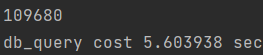
\includegraphics[height=1.1cm]{./dta/dbquery.png}}
		\caption{数据库查询}
	\end{subfigure}
	\qquad\quad
	\begin{subfigure}[b]{0.3\textwidth}
		\centerline{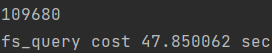
\includegraphics[height=1.1cm]{./dta/fsquery.png}}
		\caption{文件系统查询}
	\end{subfigure}
	\label{fig:visual_smap}
\end{figure*}

\par 上图所示进行十次查询并计时的结果,查询结果109680项。其中数据库每次查询平均耗时0.56s,仅为文件系统查询(平均耗时4.79s)的11.7\%。查看DBMS的查询规划可以发现,其用了如Hash join、Parallel sequence scan等技术节省时间,而在代码量相似的实现文件系统查询时仅相当于多个Sequence scan的嵌套。事实上,查询越复杂(指必要性上的复杂,而非故意将查询方式写得复杂而难以优化),DBMS的性能优势越明显(尤其是当能应用包括后面讨论的Index技术时),简单的查询可能已经难以进一步优化,性能将与文件系统相近。\\~\\
\centerline{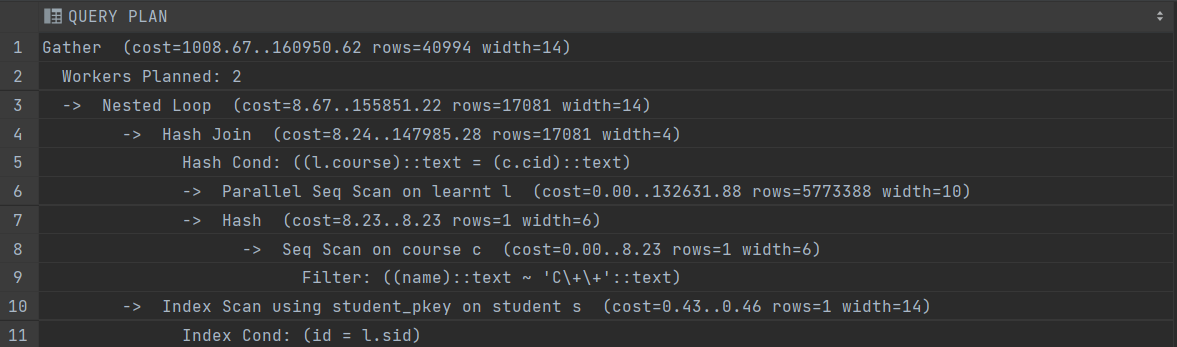
\includegraphics[width=0.9\textwidth]{dta/queryp}}
